%%%%% Set text body and margins 
%%
\documentclass[11pt]{article}
\usepackage[dvips]{graphicx,color}
\usepackage{longtable}
\usepackage{hyperref}
\usepackage{breakurl}
\hypersetup{pdfborder={0 0 100}}
%\textwidth{16.5cm}
\setlength{\textwidth}{15.5cm}
%\setlength{\textheight}{22.2cm}
\setlength{\hoffset}{-.25in}
%\setlength{\voffset}{-.9in}

\begin{document}

%%%%% The following lines create the E01-012 Technical Note Title Page
%%
\thispagestyle{empty}
\renewcommand{\thefootnote}{\fnsymbol{footnote}}

%%%%% Substitute your Note number, month and year in the following:
%%
\begin{flushright}
{\small
$b_1$ technical note 2013-05\\
May 2013\\}
\end{flushright}

\vspace{.8cm}

%%%%% Title and Author Information:
%%
\begin{center}
{\bf\large   
Rates and Statistical Uncertainty Calculations for a Measurement of $A_{zz}$}
\vspace{1cm}


E. Long (UNH), O. Rondon (INPP-UVA), P. Solvignon (Jefferson Lab)\\

\end{center}

%\vfill
\vspace{2.0cm}

\begin{center}
{\bf\large   
Abstract }

A proposal on measuring the deuteron structure function $b_1^d$ was submitted to PAC 40. The asymmetry $A_{zz}$ will be used to extract $b_1^d$. This tech note provides details on the calculations of the rates and statistical uncertainties completed for the proposal. 
\end{center}
\newpage
%\begin{quote}
%Summary of target mass corrections methods.
%\end{quote}

%\vfill

%%%%%%%%%%%%%%%
%% Choose"Presented at," "Contributed to" for conference papers
%% or "Submitted to" for journal papers
%%%%%%%%%%%%%%%
%\begin{center} 
%{\it (Invited talk presented at)} 
%   OR 
%{\it (Contributed to)} 
%(Text varies)
%{\it Conference Name} (spell out completely) \\
%{\it City, State, Country} (Location of Conference)\\
%{\it Month Day--Month Day, Year} 
%   (Indicate duration of conference.)\\

%OR\\

%{\it Submitted to A Journal} (Spell out name of journal.)
%\end{center}
%%
%%%%% End of title page


%%%%% Following are the commands to create the rest of the Note.
%%
%%%%% The next two lines change the line spacing to doublespace,
%%      if you should need to do that.
%%
%\renewcommand{\baselinestretch}{2}
%\normalsize

%%%%% Your paper starts here:
%%

%% To get page numbers in the rest of the paper:
%
\pagestyle{plain}

\section{Method of Measuring $A_{zz}$}

The deuteron cross section can be utilized to extract the tensor asymmetry, $A_{zz}$. The cross section takes the form
\begin{eqnarray}
 \frac{d^2\sigma_{\mathrm{D}}}{d\Omega dE'} = \sigma_{\mathrm{D}} = \sigma_{\mathrm{D}}^u\left[ 1  - P_z P_B A_{\parallel} + \frac{1}{2}P_{zz}A_{zz}^d \right],
\label{xs} 
\end{eqnarray}
where $\sigma_{\mathrm{D}}^u$ is the unpolarized deuteron cross section, $P_B$ is the polarization of the electron beam, $P_z$ is the vector polarization of the target, and $P_{zz}$ is the tensor polarization of the target. In the case of an unpolarized beam, the middle term vanishes leaving just
\begin{eqnarray}
\sigma_{\mathrm{D}} = \sigma_{\mathrm{D}}^u \left[1 + P_{zz} A_{zz}\right].
\label{xsbis} 
\end{eqnarray}

For the proposed measurement of $A_{zz}$, we are looking in the DIS region. The general form of DIS electron scattering off of a nucleus is described by
\begin{eqnarray}
\frac{d^2\sigma^u_X}{d\Omega dE'} = \sigma^u_X = A_X \left( \frac{d\sigma}{d\Omega} \right) _{\mathrm{Mott}_{\mathrm{p}}} \left[ \frac{2\cdot \left(\frac{F_1^{X}}{A_X} \right)}{m_{p}}\tan^2\left( \frac{\theta_{e'}}{2} \right) + \frac{\left( \frac{F_2^X}{A_X}\right) }{\nu} \right],
\end{eqnarray}
where $A_X$ is the number of nucleons, $F_1^X$ and $F_2^X$ are the nuclear structure functions, $\theta_{e'}$ is the electron scattering angle, $m_p$ is the mass of a proton, $\nu$ is the energy transfer, and $\left( \frac{d\sigma}{d\Omega} \right) _{\mathrm{Mott}_{\mathrm{p}}}$ is the Mott cross section of a proton.

In order to reduce systematic effects, a ratio of cross section is used to determine $A_{zz}$. This ratio, in terms of the measured counts with the target tensor-polarized and unpolarized, is expressed as
\begin{eqnarray}
\frac{N_{Pol}}{N_{u}} - 1 = f \frac{1}{2} A_{zz}  P_{zz},
\end{eqnarray}
where $N_{Pol}$ is the number of events recorded when the target is polarized, $N_u$ is the number of events recorded when the target is unpolarized, and a dilution factor, $f$, is included since the target material will contain nitrogen and helium as well as deuterium. Thus, $A_{zz}$ is measured through
\begin{eqnarray}A_{zz} = \frac{2  }{f \cdot P_{zz}}\left( \frac{N_{Pol}}{N_{u}} - 1 \right).
\end{eqnarray}

\section{Rates}
\label{rates-sec}
\subsection{General Expressions}

The total rates for ND3 are:
\begin{eqnarray}
R_{\mathrm{Total}}   &=& \mathcal{A}\left[ \mathcal{L}_{\mathrm{He}} \sigma_{\mathrm{He}}  + \mathcal{L}_{\mathrm{N}} \sigma_{\mathrm{N}} + \mathcal{L}_{\mathrm{D}} \sigma_{\mathrm{D}} \right]  \\
        &=& \mathcal{A}\left[ \mathcal{L}_{\mathrm{He}} \sigma_{\mathrm{He}}^u  + \mathcal{L}_{\mathrm{N}} \sigma_{\mathrm{N}}^u + \mathcal{L}_{\mathrm{D}} \sigma_{\mathrm{D}}^u\left( 1 + \frac{1}{2}P_{zz}A_{zz}^d \right) \right] 
\label{rt} 
\end{eqnarray}
where ${\cal A}$ is the acceptance ($\Delta \Omega \Delta E'$), $\sigma^u_A$ is the unpolarized cross section of the given nucleus, and $\mathcal{L}_A$ is the luminosity. The general form of the luminosity is
\begin{eqnarray}
\mathcal{L}_A = N_e \cdot {\cal N} \frac{\rho_A}{M_A} z_A p_{f_A},
\label{lumi}
\end{eqnarray}
where $N_e = I_{beam} / e$ is the rate of incident electrons, $\cal N$ is Avogadro's number, $\rho_A$ is the density, $M_A$ is the atomic or molecular mass, $z$ is the target thickness, and $p_{f_A}$ is the packing fraction of the material. Since we are using solid deuterated ammonia beads surrounded by liquid helium, the luminosities come out to
\newline
\begin{eqnarray}
\mathcal{L}_{\mathrm{He}} &=& \left[ \mathcal{N}  \frac{\rho_{\mathrm{He}}}{M_{\mathrm{He}}}\left(1 - p_f\right) \right] \cdot \left( \frac{I_{\mathrm{beam}}}{e} \right) \cdot z_{\mathrm{tgt}}, \\
\mathcal{L}_{\mathrm{N}} &=& \left[ \mathcal{N}  \frac{\rho_{\mathrm{ND}_3}}{M_{\mathrm{ND}_3}} p_f \right] \cdot \left( \frac{I_{\mathrm{beam}}}{e} \right) \cdot z_{\mathrm{tgt}},\hspace{5pt}\mathrm{and} \\
\mathcal{L}_{\mathrm{D}} &=& 3\left[ \mathcal{N}  \frac{\rho_{\mathrm{ND}_3}}{M_{\mathrm{ND}_3}} p_f \right] \cdot \left( \frac{I_{\mathrm{beam}}}{e} \right) \cdot z_{\mathrm{tgt}}. 
\label{la}
\end{eqnarray}
The factor of 3 in the expression of $\cal L_{\rm D} $ takes into account that there are three deuterium atoms in the ammonia molecule.

We will be detecting events from two different target states: polarized and unpolarized. The total rate when the target is tensor-polarized is written as
\begin{eqnarray}
R_{\mathrm{Total}}^{Pol} = \mathcal{A}\left[ \mathcal{L}_{\mathrm{He}} \sigma_{\mathrm{He}}^u  + \mathcal{L}_{\mathrm{N}} \sigma_{\mathrm{N}}^u + \mathcal{L}_{\mathrm{D}} \sigma_{\mathrm{D}}^u\left( 1 + \frac{1}{2}P_{zz}A_{zz}^d \right) \right] 
\end{eqnarray}
 and when the target is unpolarized,
 \begin{eqnarray}
R_{\mathrm{Total}}^{u} = \mathcal{A}\left[ \mathcal{L}_{\mathrm{He}} \sigma_{\mathrm{He}}^u  + \mathcal{L}_{\mathrm{N}} \sigma_{\mathrm{N}}^u + \mathcal{L}_{\mathrm{D}} \sigma_{\mathrm{D}}^u \right]. 
\end{eqnarray}
The total number of counts in each state would depend on the amount of time spent in each, such that
\begin{eqnarray}
N_{Pol} &=& R_{\mathrm{Total}}^{Pol}t_{Pol}\hspace{5pt}\mathrm{and} \\
N_{u} &=& R_{\mathrm{Total}}^{u}t_{u}.
\end{eqnarray}


\subsection{Expression of the Measured Asymmetry}

From Refs.~\cite{meyer} and \cite{uvatn}, the enhancement of the  tensor polarization with solid polarized targets can be done via the ''hole burning`` method by pushing down either one of the $|m_z|$ = 1 states moving its population to $m_z$ = 0. But this necessarily enhances the absolute vector polarization, $|m_+ - m_-|$ because one of the $m_1$'s stays fixed. So, as it is said in Ref.~\cite{meyer}, the improvement in $P_{zz}$ comes only from better $P_z$. 

In order to reduce systematic uncertainties, we find $A_{zz}$ by measuring the ratio of events detected when the target is polarized with $P_{zz}>0$ and when it is unpolarized. In terms of the rates for each state, this ratio is written
\begin{eqnarray}
\frac{N_{Pol}}{N_u} = \frac{\mathcal{A}\left[ \mathcal{L}_{\mathrm{He}} \sigma_{\mathrm{He}}^u  + \mathcal{L}_{\mathrm{N}} \sigma_{\mathrm{N}}^u + \mathcal{L}_{\mathrm{D}} \sigma_{\mathrm{D}}^u\left( 1 + \frac{1}{2}P_{zz}A_{zz}^d \right) \right] t_{Pol}}{ \mathcal{A}\left[ \mathcal{L}_{\mathrm{He}} \sigma_{\mathrm{He}}^u  + \mathcal{L}_{\mathrm{N}} \sigma_{\mathrm{N}}^u + \mathcal{L}_{\mathrm{D}} \sigma_{\mathrm{D}}^u \right] t_u },
\end{eqnarray}

\begin{eqnarray}
\frac{N_{Pol}}{N_u} = \left( \frac{t_{Pol}}{t_u}\right) \left[1 + \left( \frac{\mathcal{L}_{\mathrm{D}}\sigma_{\mathrm{D}}^u}{ \mathcal{L}_{\mathrm{He}} \sigma_{\mathrm{He}}^u  + \mathcal{L}_{\mathrm{N}} \sigma_{\mathrm{N}}^u + \mathcal{L}_{\mathrm{D}}\sigma_{\mathrm{D}}^u } \right) \frac{1}{2} A_{zz}  P_{zz}\right].
\end{eqnarray}
The luminosity terms make up the dilution factor, such that $f=\frac{\mathcal{L}_{\mathrm{D}}\sigma_{\mathrm{D}}^u}{ \mathcal{L}_{\mathrm{He}} \sigma_{\mathrm{He}}^u  + \mathcal{L}_{\mathrm{N}} \sigma_{\mathrm{N}}^u + \mathcal{L}_{\mathrm{D}}\sigma_{\mathrm{D}}^u }$ and

\begin{eqnarray}
\frac{N_{Pol}}{N_u} = \left( \frac{t_{Pol}}{t_u}\right) \left[1 + f \frac{1}{2} A_{zz}  P_{zz}\right].
\end{eqnarray}

If equal time is spent on each polarization state such that $t_{Pol} \approx t_u$, then
\begin{eqnarray}
\frac{N_{Pol}}{N_u} =  1 + f \frac{1}{2} A_{zz}  P_{zz}.
\end{eqnarray}
This can be split up into a measured ratio, $A_{\mathrm{meas}}$, defined as
\begin{eqnarray}
A_{\mathrm{meas}} = \frac{N_{Pol}}{N_u} - 1.
\end{eqnarray}
From this, $A_{zz}$ can be extracted by
\begin{eqnarray}
A_{zz} = \frac{2  }{f \cdot P_{zz}}A_{\mathrm{meas}}.
\end{eqnarray}




\begin{table}[htdp]
\caption{Values used in the rate estimates.}
\begin{center}
\begin{tabular}{|c|c|}
\hline
$\rho_{\rm ND_3}$	&	1.007 g.cm$^{-3}$ \\
$M_{\rm ND_3}$		&	20 g.mol$^{-1}$ \\
$p_f({\rm ND_3})$	&	0.65 \\
$z_{\mathrm{tgt}}$	&	3 cm \\
$P_{zz}$				&	0.25 \\
\hline
\end{tabular}
\end{center}
\label{default}
\end{table}%

\section{Statistical Uncertainty}
\label{stat-sec}

Given the form of $A_{zz}$ in terms of $A_{\mathrm{meas}}$, 
\begin{eqnarray}
A_{zz} = \frac{2  }{f \cdot P_{zz}}A_{\mathrm{meas}},
\end{eqnarray}
we can find the uncertainty from
\begin{equation}
\delta A_{zz} = \sqrt{\left( \frac{\partial A_{zz}}{\partial A_{\mathrm{meas}}} \delta A_{\mathrm{meas}} \right)^2 + \left( \frac{\partial A_{zz}}{\partial f} \delta f \right)^2 + \left( \frac{\partial A_{zz}}{\partial P_{zz}} \delta P_{zz} \right)^2 }.
\end{equation}
In this case, we can break it down into statistical and systematic uncertainties,
\begin{equation}
\delta A_{zz} = \sqrt{\left( \delta A_{zz}^{\mathrm{Stat}} \right) ^2 + \left( \delta A_{zz}^{\mathrm{Sys}} \right) ^2 }.
\label{azz_err}
\end{equation}
The statistical component relates as
\begin{equation}
\delta A_{zz}^{\mathrm{Stat}} = \frac{\partial A_{zz}}{\partial A_{\mathrm{meas}}} \delta A_{\mathrm{meas}} = \frac{2}{f\cdot P_{zz}} \delta A_{\mathrm{meas}}.
\end{equation}
Since $A_{\mathrm{meas}} = \frac{N_{Pol}}{N_u} - 1$, the uncertainty in $A_{\mathrm{meas}}$ depends on the number of events counted in each state as described by
\begin{equation}
\delta A_{\mathrm{meas}} = \sqrt{ \left( \frac{\partial A_{\mathrm{meas}}}{\partial N_{Pol}} \delta N_{Pol} \right)^2 + \left( \frac{\partial A_{\mathrm{meas}}}{\partial N_{u}} \delta N_{u} \right)^2 },
\end{equation}
\begin{equation}
\delta A_{\mathrm{meas}} = \sqrt{ \left( \frac{1}{N_u} \sqrt{N_{Pol}} \right)^2 + \left( -\frac{N_{Pol}}{N_u^2} \sqrt{N_u} \right)^2 },
\end{equation}
\begin{equation}
\delta A_{\mathrm{meas}} = \sqrt{  \frac{N_{Pol}}{N_u^2} + \frac{N_{Pol}^2}{N_u^3}  }.
\end{equation}

Because $A_{zz}$ is very small, we can assume that $N_{Pol} \approx N_u \approx \frac{N}{2}$, then
\begin{equation}
\delta A_{\mathrm{meas}} = \sqrt{  \frac{N/2}{N^2/4} + \frac{N^2/4}{N^3/8}  },
\end{equation}
\begin{equation}
\delta A_{\mathrm{meas}} = \frac{2}{\sqrt{N}}.
\label{ameas_err}
\end{equation}
Equation (\ref{ameas_err}) can be put back into equation (\ref{azz_err}) to get
\begin{equation}
\delta A_{zz}^{\mathrm{Stat}} = \frac{2}{f\cdot P_{zz}} \left( \frac{2}{\sqrt{N}} \right),
\end{equation}
\begin{equation}
\delta A_{zz}^{\mathrm{Stat}} = \frac{4}{f\cdot P_{zz}\sqrt{t\cdot R_{\mathrm{Total}}}}.
\end{equation}



\section{Kinematics}
\label{kine-sec}
In order to determine the kinematics to be used, a balance was struck between the physical constraints of the detector, increasing the rate by moving to a lower angle, and maximizing the number of events occurring from DIS. The kinematics selected for this technote are described in Table \ref{tab:kine}.


\begin{table}[htdp]
\caption{Central values of the kinematics chosen for the $b_1$ proposal.}
\begin{center}
\begin{tabular}{|c|c|c|c|c|c|c|}
\hline
   Detector & $x$  &   $Q^2$ &    $W$  &  $E_{e'}$  &  $\theta_{e'}$  &  $\theta_q$ \\
\hline   
SHMS	 & 0.15 &	1.21 & 2.78 & 6.70 &  7.35 & 11.13 \\
SHMS	 & 0.30 &	2.00 & 2.36 & 7.45 &  8.96 & 17.66 \\
SHMS	 & 0.45 &	2.58 & 2.00 & 7.96 &  9.85 & 23.31 \\
HMS	 & 0.55 &	3.81 & 2.00 & 7.31 & 12.50 & 22.26 \\
\hline  
\end{tabular}
\end{center}
\label{tab:kine}
\end{table}%

Estimates for the total kinematic range were calculated in a FORTRAN code, discussed in Section \ref{results-sec}, which looked at the entire acceptance range of the HMS and SHMS. These ranges are displayed in Figure \ref{fig-kine}.

\begin{figure}
	\begin{center}
	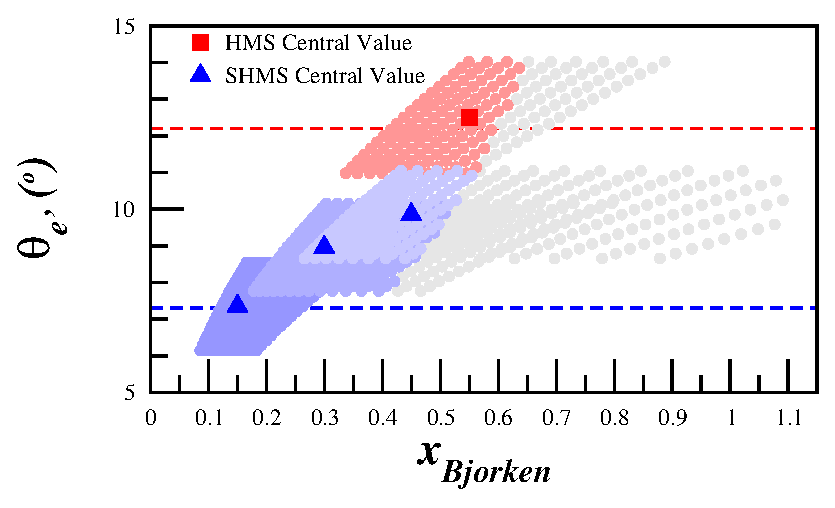
\includegraphics[width=6cm]{hms_shms_theta.eps} \hspace{10px} 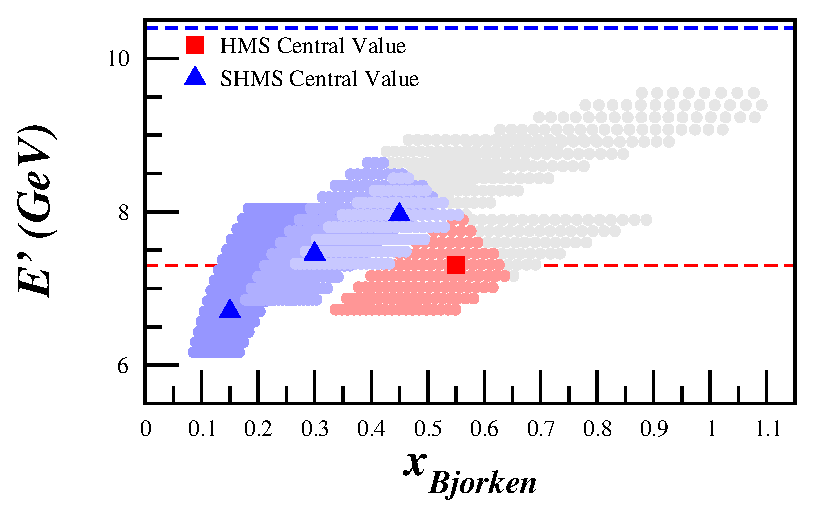
\includegraphics[width=6cm]{hms_shms_eprime.eps}	
	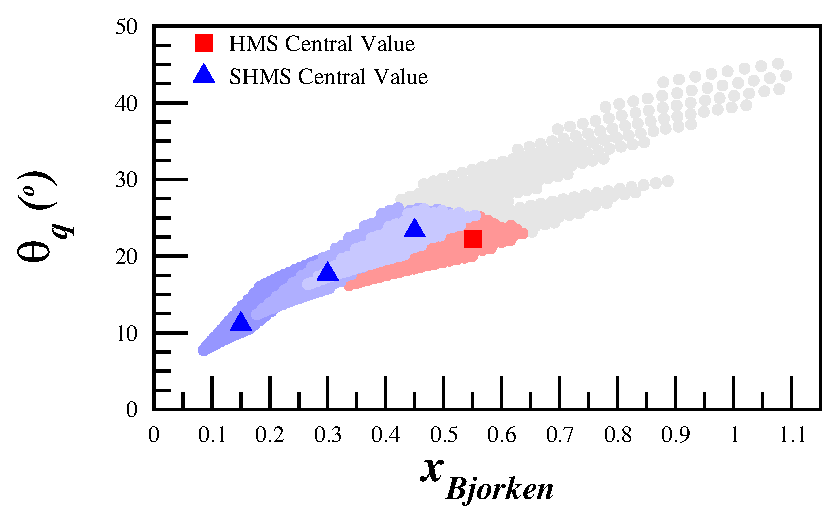
\includegraphics[width=6cm]{hms_shms_theta_q.eps} \hspace{10px} 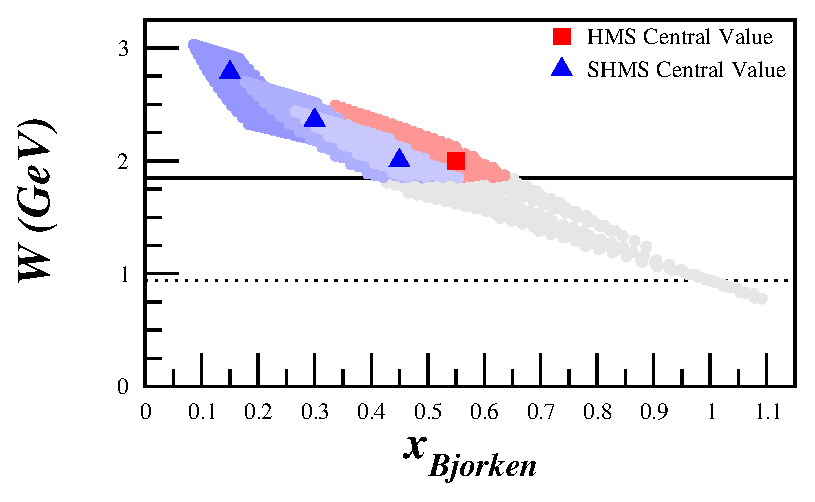
\includegraphics[width=6cm]{hms_shms_w.eps}	
	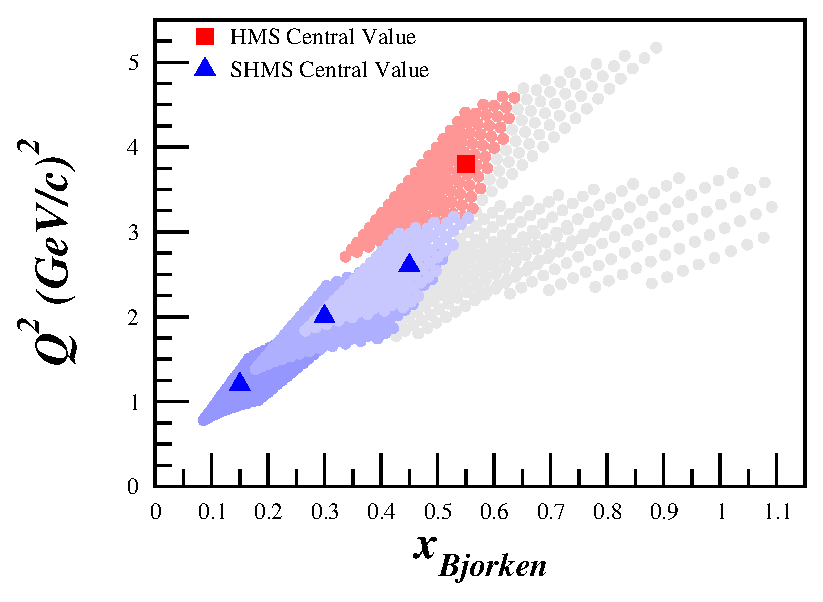
\includegraphics[width=6cm]{hms_shms_q2.eps}	
	\end{center}
	\caption [Kinematics] {Kinematics chosen for the HMS and SHMS. The darker colored points indicate the central HMS or SHMS value, the red (blue) dotted lines represent the limits of the central value of the HMS (SHMS), and the light grey represent events that will be cut to ensure that DIS is held by maintaining $W>1.85$ GeV, shown as a solid black line.}
	\label{fig-kine}
\end{figure}

\newpage 
\section{Calculated Systematic Uncertainties}
\label{results-sec}
Code was written by P. Solvignon and E. Long to automate the method described in Sections \ref{rates-sec} and \ref{stat-sec} using the kinematics discussed in Section \ref{kine-sec}. The FORTRAN code used is available at \url{http://nuclear.unh.edu/~elong/analysis_files/2013-05-09/b1_rates-2013-05-09.tar.gz}. It takes the weighted cross-sections for each kinematics setting and uses it to estimate both the rates and the statistical uncertainty in $A_{zz}$. The rates and the amount of time spent at each setting, assuming 100\% efficiency, are presented in Figure \ref{fig:rates}.

\begin{figure}
	\begin{center}
	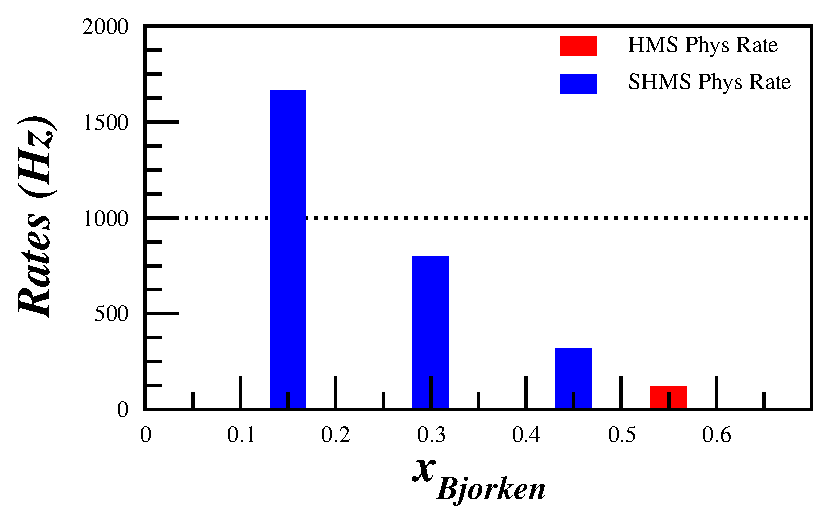
\includegraphics[width=6cm]{hms_shms_rates.eps} \hspace{10px} 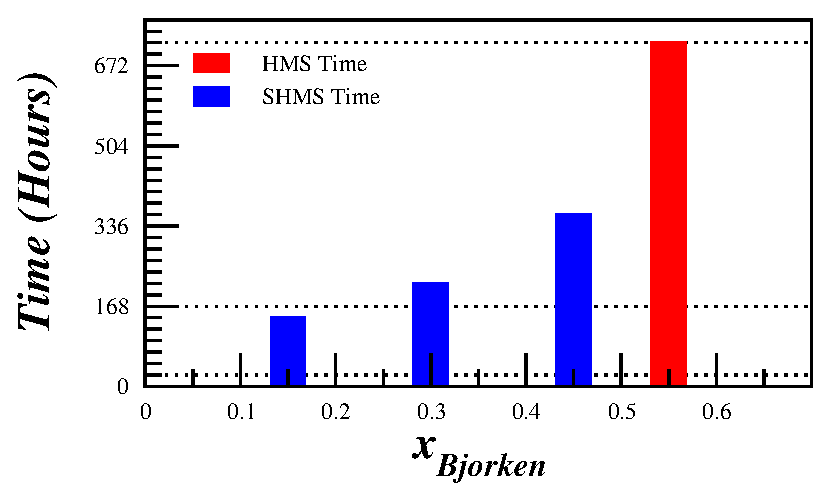
\includegraphics[width=6cm]{hms_shms_time.eps}	
	\end{center}
	\caption [Rates and Time] {The calculated rates are presented alongside the amount of time, assuming 100\% efficiency, that was used to estimate the uncertainty in $A_{zz}$ and $b_1^d$.}
	\label{fig:rates}
\end{figure}


Since many of the spectrometer settings overlap in $x$, as shown in Figure \ref{fig-kine}, the number of events in each $x$ bin were integrated so that a distinct measurement of $A_{zz}$ against $x$ could be made. The calculated uncertainty in $A_{zz}$ is shown in Figure \ref{fig-dAzz}.

\begin{figure}
	\begin{center}
	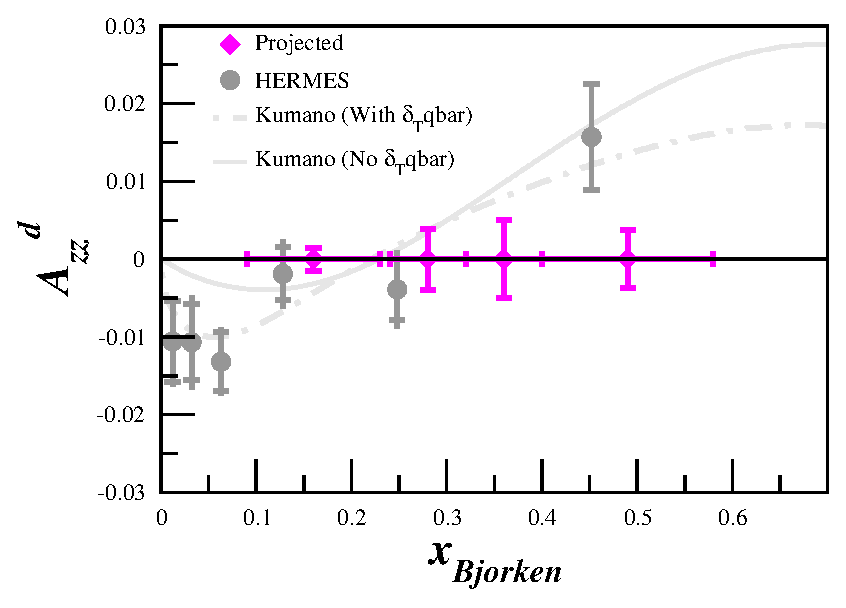
\includegraphics[width=8cm]{hms_shms_Azz.eps}
	\end{center}
	\caption [Uncertainty in $A_{zz}$] {The estimated uncertainty in $A_{zz}$ is plotted against previous data by HERMES and a number of theoretical calculations.}
	\label{fig-dAzz}
\end{figure}


Additionally, it estimates the uncertainty on $b_1^d$, which is extracted from $A_{zz}$ by
\begin{equation}
b_1^d = - \frac{3}{2}A_{zz} \left( \frac{F_1^d}{A_{\mathrm{D}}} \right)= - \frac{3}{2}A_{zz} \left( \frac{F_1^d}{2} \right). 
\end{equation}
The systematic uncertainty on $b_1^d$ is dependent on the uncertainty in $A_{zz}$ such that 
\begin{equation}
\delta b_1^d =\sqrt{ \left[ - \frac{3}{2} \left( \frac{F_1^d}{2} \right)\delta A_{zz} \right]^2}.
\end{equation}
This uncertainty was also calculated, based on the statistical uncertainty on $A_{zz}$, and is show in Figure \ref{fig-db1}.

\begin{figure}
	\begin{center}
	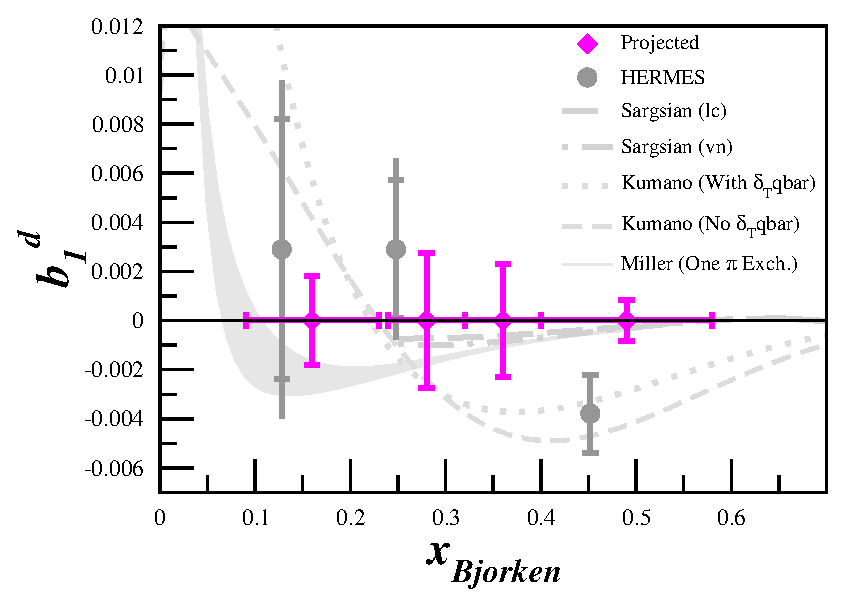
\includegraphics[width=8cm]{hms_shms_b1.eps}
	\end{center}
	\caption [Uncertainty in $b_1^d$] {The estimated uncertainty in $b_1^d$ is plotted against previous data by HERMES and a number of theoretical calculations.}
	\label{fig-db1}
\end{figure}



%\section{Systematics}

%%%%% Acknowledgments

%\section*{Acknowledgments}

%
\newpage
%%%%% Bibliography
%%
\begin{thebibliography}{6}

\bibitem{meyer} T.W.~Meyer and E.P.~Schilling, Tensor polarized deuteron targets for intermediate energy physics experiments, BONN-HE-85-06 (1985)

\bibitem{uvatn} S.~Bueltmann, D.~Crabb, Y.~Prok. UVa Target Studies, UVa Polarized Target Lab technical note, 1999.

%\bibitem{BITAR} K. Bitar, P. W. Johnson and W.-K. Tung, Phys. Lett. {\bf B83}, 114 (1979)

%\bibitem{WALLY} W. Melnitchouk and F. M. Steffens (work in progress)

%\bibitem{ELLIS} R. K. Ellis, W. Furmanski and R. Petronzio, Nucl.Phys. {\bf B212}, 29 (1983)

%\bibitem{QIU} A. Accardi and J.-W. Qiu (work in progress)

\end{thebibliography} 
%%
%%%%% End Bibliography

\end{document}
%%
%%%%% End tech_note.tex
%%%%% EOF



